% !TEX root = ./main.tex
%\section{Key properties of criticality}
%\label{sec:structure}
%We describe connections
%between the proposed problems and Influence
%Maximization, which will have implications on the computational complexity.
%We also prove structural properties of these objectives, later used in our algorithms.


%\section{Hardness of $k$-\maxcrit}
\subsection{Computational Complexity}
\maxcrit{} is related to the classical Influence Maximization (IM) problem \cite{kempe:sigkdd03}. Briefly, in IM, we are given a directed graph, disease transmission probabilities for each edge, and a size constraint $k$. The goal is to find a \emph{seed set} of $k$ nodes to be the source of an infection, such that the number of infected nodes, following a given disease model, is maximized. \maxcrit{} may be seen as a generalization of IM with a connectivity constraint on the seed set. %Based on this relationship, we can derive the computational complexity of \maxcrit{}.
Based on this relationship, one can show that \maxcrit{} is NP-hard, just as IM. However, as discussed below, the connectivity constraint makes our target problem algorithmically more challenging.

%\begin{theorem}
%\label{theorem:nphard}
%\emph{MaxCrit} is NP-hard.
%\end{theorem}
%\begin{proof}
%By reduction from Influence Maximization (Supplementary Material).
%\end{proof}

\subsection{Impact of connectivity requirement}
Though \maxcrit{} is closely related to IM, we cannot directly apply the current methods for IM. This is because the connectivity constraint has a strong effect on the solution of \maxcrit{}. A solution computed for \infmax{} using the greedy algorithm of \cite{kempe:sigkdd03} can be arbitrarily suboptimal for \maxcrit{}. Informally, this follows because, in \infmax{}, it is better to choose seeds that are far apart and disconnected, so that their combined number of infections is maximized.

\begin{observation}
\label{obs:infmax}
There exists a family of instances $(G, H_{\R}, k)$ for which the optimum solution
$S^*$ to \maxcrit{} satisfies
$\maxcrit(S^*) =O(\frac{1}{k}\infmax(\hat{S}))$, where $\hat{S}$ is the optimum
solution to the \infmax{} version for this instance, without any connectivity requirements.
\end{observation}

For example, consider a cycle graph, as in Figure \ref{fig:observation}. Every node has one outgoing neighbor (clockwise direction), and every node infects its neighbor with probability 1, unless the neighbor is a blue node, in which case the probability is 0, as denoted in the figure. There are $k=4$ spreader nodes (in blue) separated by paths of length $k+1$. Consider an instance of $\infmax{}$ with size constraint $k$, and the analogous instance of $\maxcrit{}$, where, for simplicity, we assume that $G = \HR$. The optimal solution to \infmax{} consists of the $k$ hub nodes, with objective value equals to the number of nodes in the graph, $k(k+1)$, since each hub is able to propagate the infection through all the white nodes until the next clockwise hub. In contrast, the solution to \maxcrit{} must be a connected set of nodes, so the best solution would consist of a hub and the next $k$ clockwise white nodes, for an objective value of $k + 1$.

\begin{figure}
    \centering
    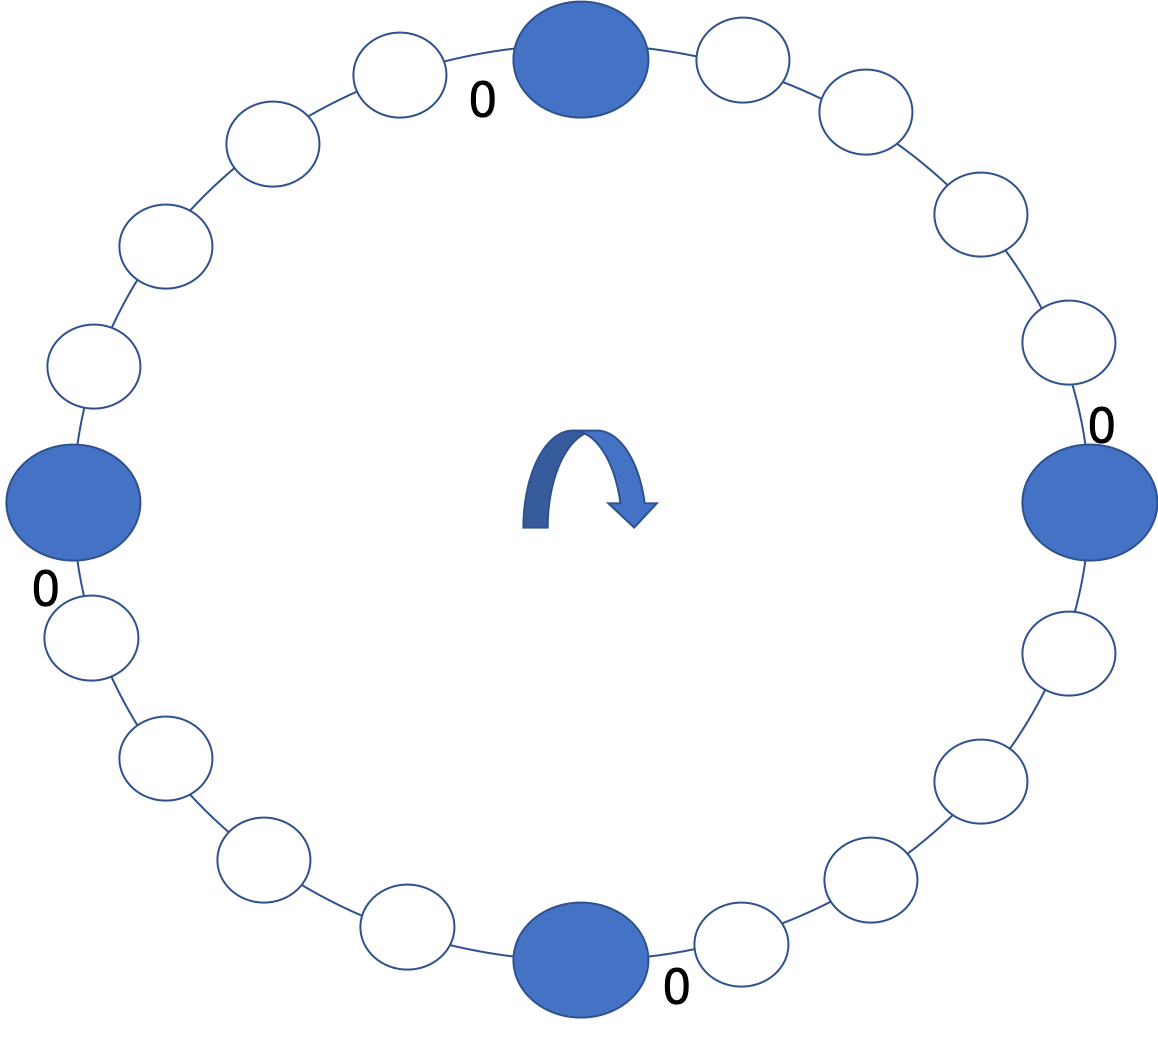
\includegraphics[width=.5\columnwidth]{img/observation.png}
    \caption{Effect of connectivity constraint in cycle graph with $k=4$ spreader nodes (blue) separated by paths of length $k + 1$. The optimal solution to $\infmax{}$ has $k$ times the objective value of the optimal solution for \maxcrit{}. See text for details.}
    \label{fig:observation}
\end{figure}

%\subsection{Submodularity of \maxcrit{} and \avgcrit{}}
%\label{sec:submodular}
%A set function $f: 2^V \rightarrow \mathbb{R}$ is said to be \emph{submodular} if it satisfies the diminishing returns property: for any $T \subset S\subset V$ and $x \in V\setminus S$, we have that $f(T \cup \{x\}) - f(T) \geq f(S \cup \{x\}) - f(S)$. In recent years, there has been notable interest in submodularity as a key property to approach problems in machine learning. We exploit this property to design efficient algorithms for the proposed problems.%We have the following result:
%
%\begin{lemma}
%\label{lemma:submodular}
%$\maxcrit{}$ and $\avgcrit{}$ are submodular.
%\end{lemma}

%\begin{proof}
%Consider a random live graph $L(V, E')$ defined as above, and let $\crit_{L}(S, \mathbf{x})$ be the criticality of $S\subset V$ on this graph. Without loss of generality, assume there is only one initial infection and let $r$ be the initially infected node. Then, the criticality of $S$ can be computed as
%$$
%\crit_L(S, \mathbf{x}) = |\left(\bigcup_{s \in S} \text{comp}_L(s)\right) \cup \text{comp}_L(r)| - |\text{comp}_L(r)|.
%$$
%In words, the number of extra infections in $L$ due to node set $S$ is the size of the union of the components of nodes in $S$ minus the infections that we get if only the seed is infected---i.e., the size of $\text{comp}_L(r)$.
%
%Now, consider two sets $S,T$, such that $T\subseteq S$, and a node $v \not \in S$. The quantity $\crit_L(T \cup \{v\}, \mathbf{x}) - \crit_L(T, \mathbf{x})$ is the number of extra infections from adding node $v$; that is, the number of elements in $\text{comp}_L(v)$ that are not already in $(\bigcup_{s \in T} \text{comp}_L(s)) \cup \text{comp}_L(r)$. This number is at least as large as the number of extra infections that we get by adding $v$ to the bigger set $S$, which gives us $\crit_L(T \cup \{v\}, \mathbf{x}) - \crit_L(T, \mathbf{x}) \geq \crit_L(S \cup \{v\}, \mathbf{x}) - \crit_L(S, \mathbf{x})$. This is precisely the definition of submodularity, so the criticality function for a fixed graph is submodular. Over random realizations of $L$, we obtain
%$$
%\crit(S, \mathbf{x}) = \sum_{L}\text{Pr}(L) \crit_L(S, \mathbf{x}).
%$$
%This is a convex combination of submodular functions, which is known to be submodular too, completing the proof.
%\end{proof}

%We present the proof in the Supplementary Material. The argument is similar to the submodularity proof for \infmax{}.

\section{Proposed Methods}
\label{sec:proposed-critical}
Our strategy involves showing that the $\crit$ function is submodular; then, the $\maxcrit{}$ problem reduces to maximizing a submodular function over connected subgraphs of $\HR$. We start with the necessary definitions.

\subsection{Submodular function maximization with connectivity constraints}
\label{sec:submod-connectivity}
A set function $f: 2^{\R} \rightarrow \mathbb{R}$ is said to be \emph{submodular} if it satisfies the diminishing returns property: for any $S \subset S'\subset \R$ and $x \in \R\setminus S'$, we have that $f(S \cup \{x\}) - f(S) \geq f(S' \cup \{x\}) - f(S')$. That is, we obtain a larger increase in $f$ when adding an element $x$ to a smaller set. In recent years, there has been notable interest in submodularity as a key property to approach problems in machine learning \cite{krause2008beyond}. 

Here, we consider $f(S)=\crit(S, \mathbf{x}, \src)$. For notational simplicity, we will drop $\mathbf{x}$ and $\src$. Our first key result is that $\crit$ is submodular. %(proof in the Supplementary Material).

\begin{lemma}
$\text{\emph{\crit(}S\text{\emph{)}}}$ is a submodular function of $S\subset\R$.
\end{lemma}

\begin{proof}
We follow the approach of Kempe et al.\ \cite{kempe:sigkdd03}, who analyze one random realization of the diffusion process at a time. For simplicity, we prove the submodularity of $\crit$ for the Independent Cascade model, but the result extends to the more general SEIR process. For each edge $e=(u,v)$, we flip a coin with bias equal to the transmission probability $p(u,v)$. Let $X(e)$ be a Bernoulli variable that is 1 with probability $p(u,v)$; then, we define the \emph{live} graph $L(V, E')$ as the subgraph of $G$ induced by the edges for which $X(e) = 1$: $L' = (V, E'=\{e \in E | X(e) = 1\})$. In the live graph, a node $v$ is infected by the end of the diffusion process if and only if $v$ is in the same component as one of the seeds in $S$. Without loss of generality, assume there is only one initial infection and let $r$ be the initially infected node. Then, the criticality of $S$ can be computed as
$$
\crit_L(S) = \left|\left(\bigcup_{s \in S} \text{comp}_L(s)\right) \cup \text{comp}_L(r)\right| - \left|\text{comp}_L(r)\right|.
$$
In words, the number of extra infections in $L$ due to node set $S$ is the size of the union of the components of nodes in $S$ minus the infections that we get if only $r$ is infected---i.e., the size of $\text{comp}_L(r)$.

Now, consider two sets $S,T$, such that $T\subseteq S$, and a node $v \not \in S$. The quantity $\crit_L(T \cup \{v\}) - \crit_L(T)$ is the number of extra infections from adding node $v$; that is, the number of elements in $\text{comp}_L(v)$ that are not already in $(\bigcup_{s \in T} \text{comp}_L(s)) \cup \text{comp}_L(r)$. This number is at least as large as the number of extra infections that we get by adding $v$ to the bigger set $S$, which gives us $\crit_L(T \cup \{v\}) - \crit_L(T) \geq \crit_L(S \cup \{v\}) - \crit_L(S)$. This is precisely the definition of submodularity, so the criticality function for a fixed live graph is submodular. Over random realizations of $L$, we obtain
$$
\crit(S) = \sum_{L}\text{Pr}(L) \crit_L(S).
$$
where $\text{Pr}(L)$ denotes the probability of obtaining the live graph $L$ with the edge probabilities $p(u,v)$. This is a convex combination of submodular functions, which is known to be submodular too, completing the proof.
\end{proof}

The \maxcrit{} problem can be seen as maximizing the submodular function $\crit(S)$ over all connected $S\in\ConnR$, with $|S|\leq k$. The connectivity constraint significantly increases the computational complexity of the problem. In contrast, the relaxed problem of maximizing a submodular function subject \emph{only} to a size constraint $k$ can be approximated to a constant factor. Given a submodular function $f(\cdot)$, the $\greedy{}$ algorithm of \cite{nemhauser1978analysis} finds a set $S$ with objective value at least $(1 - 1/e)$ of the optimal by iteratively adding a node $v$ to $S$ that maximizes the marginal benefit, $f(S\cup\{v\}) - f(S)$.
For submodular maximization with connectivity constraints, \cite{kuo2015maximizing} give an $\Omega(1/\sqrt{k})$ approximation guarantee. Below, we derive an improved algorithm by exploiting the geometric structure of the graph.

\subsection{Algorithm \algosubmod{}}
Recall the definitions of $B(v, \ell)$, $\dist(u, v)$, and the doubling dimension $d$. For subsets $S\subseteq T \subseteq \R$, we say that $T$ is a steiner tree spanning $S$ if the nodes in $T$---and, consequently, $S$---are connected in $\HR$. The following lemma shows that, if the nodes in a set $S$ are within some bounded distance, we can find a steiner tree spanning $S$ that is not ``too large''.

\begin{lemma}
\label{lemma:udg}
Let $\HR$ be a graph with doubling dimension $d$.
Consider any subset $S\subseteq B(r, \ell)$ for any $r\in\R$, $\ell\geq 0$.
Then, there exists a steiner tree $T$ that spans $S$, such that $|T|=O\Big(\frac{\ell^d}{\hat{\ell}^{d-1}}+|S|\hat{\ell}\Big)$, for any $\hat{\ell}\leq\ell$.
\end{lemma}
\begin{proof} 
We first observe that $B(r, \ell)$ can be covered by at most $O((\ell/\hat{\ell})^d)$ balls of radius $\hat{\ell}$. Let $\ell/\hat{\ell}=2^x$, and assume $x$ is an integer (the bound holds even if this is not the case). Since $\HR$ has doubling dimension, $B(v, \ell)$ can be covered by at most $2^d$ balls of radius $\ell/2$, $2^{2d}$ balls of radius $\ell/2^2$, and so on. Therefore, $B(r, \ell)$ can be covered by $2^{xd}=(\ell/\hat{\ell})^d$ balls of radius $\ell/2^x=\hat{\ell}$. Let $B(v_1,\hat{\ell}),\ldots,B(v_N,\hat{\ell})$ be the $N=O((\ell/\hat{\ell})^d)$ balls of radius $\hat{\ell}$ which cover $B(r, \ell)$.

Next, consider a graph $\hat{H}=(\{v_1,\ldots,v_N\},\hat{E})$, where $(v_i, v_j)\in\hat{E}$ if there exist $u\in B(v_i, \hat{\ell})$ and $u'\in B(v_j, \hat{\ell})$ such that $u, u'$ are adjacent in $\HR$. Then, for each $(v_i, v_j)\in \hat{E}$, we have $\dist_{\hat{H}}(v_i, v_j)\leq 2\hat{\ell}$. 
It also follows that $\hat{H}$ is a connected graph, since $B(r, \ell)$ is connected, and the balls centered at $v_1,\ldots,v_N$ cover it. Let $T'$ be any spanning tree of $\hat{H}$, which must exist because $\hat{H}$ is connected. Further, since $T'$ has $(N-1)$ edges from $\hat{E}$, we have $$
\sum_{(v_i, v_j)\in T'}\dist_{\hat{H}}(v_i, v_j)\leq 2\hat{\ell}(N-1)\leq 2\hat{\ell}N=O(\ell^d/\hat{\ell}^{d-1}).
$$
Let $T''$ be a tree in $\HR$ obtained by replacing each edge $(v_i, v_j)$ in $T'$ by the shortest path between $v_i$ and $v_j$ in $\HR$. By definition, the length of this path is $\dist_{\HR}(v_i, v_j)$, and so, $|T''|=O(\ell^d/\hat{\ell}^{d-1})$.

Any node $v\in S$ is within distance $\hat{\ell}$ of a node in $T''$, since there exists $v_i$ such that $v\in B(v_i, \hat{\ell})$, and $v_i\in T''$. We now construct a tree $T$ by connecting each node $v\in S$ by a shortest path to the closest node in $T''$. We have $|T|\leq |T''|+|S|\hat{\ell}$, since each such node $v$ can be connected by a path of length at most $\hat{\ell}$. From the bound on $|T''|$, we have $|T|=O(\ell^d/\hat{\ell}^{d-1}+|S|\hat{\ell})$.
\end{proof}

%The greedy algorithm of \cite{nemhauser1978analysis} in Step 2 of \algosubmod{}
%iteratively adds a node $v$ to $S$ that maximizes the marginal benefit,
%$f(S\cup\{v\}) - f(S)$. The connectivity constraints are ignored in this step.
%A Steiner tree is one that connects the nodes in $S$, possibly using additional not in $S$, referred to as the ``Steiner'' nodes (see \cite{vaz01} for definitions). An optimal Steiner tree of size at most $k$ can be computed using the algorithm of \cite{cadena:sdm17}.

The following lemma establishes that there exists a ball $B(r, \ell)$ that has a significant overlap with an optimal solution. The proof is analogous to that of Claim 2 in \cite{kuo2015maximizing}.

\begin{lemma}
\label{lemma:opt}
Let $S^*$ be an optimal solution that maximizes $\crit(\cdot)$. There exists $r\in \R$, such that for any $\ell$,
$$
\crit(S^*\cap B(r, \ell))=\Omega(\frac{\ell}{k}\crit(S^*)).
$$
\end{lemma}
% \begin{proof} (Sketch)
% Let $T^*$ be a tree that spans $S^*$. Consider an in-order traversal of $T^*$, and
% let $\{r_1,r_2,\ldots,r_m\}$ be an ordering of the nodes in this traversal. Some nodes
% might get repeated, but we have $m\leq 2k$.
% We consider a greedy covering of $S^*$ and construct a subset $\hat{S}$
% in the following iterative manner. 
% We pick each node $r_i$ in turn, and the largest radius $s_i \leq k^{2/3}$ such that 
% $|D(r_i, s_i)\cap S^*|=O(k^{2/3})$. We remove the nodes of $D(r_i, s_i)$ from
% $\{r_1,r_2,\ldots,r_m\}$, and add $D(r_i, s_i)$ to $\hat{S}$.
% It can be shown that $|\hat{S}|=O(k^{1/3})$.
% Since $\cup_{D\in \hat{S}} D \supseteq S^*$, we have
% $\sum_{D\in \hat{S}} f(D) \geq f(S^*)$. This implies that there exists
% some $D(r, s)\in \hat{S}$ such that $f(S^*\cap D(r, s))\geq \frac{1}{k^{1/3}} f(S^*)$.
% \end{proof}

We now have the tools to design \algosubmod{} (Algorithm \ref{alg:algosubmod}) for the $\maxcrit{}$ problem. As in \cite{kuo2015maximizing}, the main idea is to first solve the relaxed problem where we ignore the connectivity constraint (line 2), and then make the solution connected via a steiner tree (line 3). By combining Lemmas \ref{lemma:udg} and \ref{lemma:opt}, we obtain an improved approximation.

\begin{algorithm}{}
\caption{\small $\algosubmod(H_{\R}, k, \ell)$}
\label{alg:algosubmod}
\begin{algorithmic}[1]
\begin{small}
\FOR{$r \in H_{\R}$}
  \STATE 
%Run the $\greedy{}$ algorithm of \cite{nemhauser1978analysis}
%to pick a subset $S\subseteq B(r, \ell)$ of size $\ell$
Run $\greedy(B(r, \ell), \crit, \ell)$ to get subset $S\subseteq B(r, \ell)$ of size $\ell$
  \STATE Construct a minimum steiner tree $T(r, \ell)$ of $S$ in graph $\HR$
\ENDFOR
\STATE return $\mbox{argmax}_{r} \{\crit(T(r, \ell))\}$
\STATE
\STATE\textbf{procedure} $\greedy(V, f, k)$ \cite{nemhauser1978analysis}
%\STATE \textbf{Input}: Ground set $V$, submodular function $f$, and size parameter $k$
%\STATE \textbf{Output}: Set $S$ of size $k$, with objective value $f(S)$ at least $(1 - 1/e)$ of the optimal
\STATE Let $S = \emptyset$
\FOR{$i = 1$ to $k$}
\STATE $x = \mbox{argmax}_{x' \in V\setminus S} f(S \cup \{x'\}) - f(S)$
\STATE $S = S \cup \{x\}$
\ENDFOR
\STATE return $S$
\end{small}
\end{algorithmic}
\end{algorithm}

\begin{theorem}
\label{theorem:submod}
Let $T(r, \ell)$ be the tree returned by Algorithm \algosubmod{}, and let $\HR$ have doubling dimension $d$. Then, for $\ell=k^{\frac{d}{2d-1}}$, $\crit(T(r, \ell))=\Omega\Big(\frac{1}{k^{(d-1)/(2d-1)}} \crit(S^*)\Big)$ and $T(r, \ell)$ has size at most $2k$.
\end{theorem}
\begin{proof}
By Lemma \ref{lemma:opt}, there exists a ball $B(r, \ell)$, such that $\crit(S^*\cap B(r, \ell))=\Omega(\frac{\ell}{k}\crit(S^*))$.
The $\greedy$ subroutine picks a subset $S\subseteq B(r, \ell)$ of size at most $\ell$, such that $\crit(S)\geq(1-1/e) \crit(S^*\cap B(r, \ell)) = \Omega(\frac{\ell}{k} \crit(S^*))$.

By Lemma \ref{lemma:udg}, there is a tree $T$ spanning $S$ with $|T|=O(\ell^d/\hat{\ell}^{d-1}+|S|\hat{\ell})$.
By selecting $\ell=k^{\frac{d}{2d-1}}$ and $\hat{\ell}=k^{\frac{d-1}{2d-1}}$, we get
\begin{eqnarray*}
|T| &=&O(\ell^d/\hat{\ell}^{d-1}+|S|\hat{\ell})\\
&\leq& \frac{k^{d^2/(2d-1)}}{k^{(d-1)^2/(2d-1)}} + k^{d/(2d-1)}k^{(d-1)/(2d-1)}\\
&\leq& 2k
\end{eqnarray*}
Finally, we have 
\[
\crit(T(r, \ell))=\Omega\left(\frac{\ell}{k}\crit(S^*)\right) = \Omega\Big(\frac{1}{k^{(d-1)/(2d-1)}} \crit(S^*)\Big)
\]
\end{proof}

\noindent
\textbf{Improvement over the best-known bound of \cite{kuo2015maximizing}.} We note that, for any $d> 0$, we have $1/k^{(d-1)/(2d-1)}\geq 1/\sqrt{k}$. Since any graph has finite doubling dimension, Algorithm \algosubmod{} improves the current best bound for submodular maximization with connectivity constraints.


\subsection{Quota Steiner Tree problem}
\label{sec:algomaxst}
We also use a variation of steiner tree, referred to as Quota Steiner Tree (\textsc{QST}), as a subroutine in our algorithm. This problem is defined in the following manner \cite{Johnson2000PCS}:
given a graph $H_{\R}$, a weight $\wt_r$ for each $r\in \R$, and a parameter $k$, find a tree $T'$ in $H_{\R}$ with at most $k$ nodes, such that $\sum_{r\in T'} \wt_r$ is maximized.


In fact, \textsc{QST} is a special, easier instance of the above problem of submodular maximization with connectivity constraints, since $\sum_{r\in T'} \wt_r$ is a modular function.
There are constant factor approximations for QST \cite{ravi1996spanning}. Here, we adapt the randomized fixed-parameter tractable algorithm of \cite{cadena:sdm17}, which yields an optimal solution for \textsc{QST}  with high probability in time $O(|E|(2e)^k)$, which is a fixed parameter tractable algorithm in $k$. We refer to this algorithm as \algomaxst{}, and we find that integrating it as a subroutine in Algorithm \ref{alg:algosubmod} improves optimization power in practice.

\subsubsection{Algorithm \algomaxcrit{}}
\begin{algorithm}{}
\small
\caption{\small $\algomaxcrit(H_{\R}, k)$}
\label{alg:algomaxcrit}
\begin{algorithmic}[1]
\STATE Run Algorithm $\algosubmod(H_{\R}, k)$, and let $\hat{T}$ be the subgraph returned
\FOR{$r\in H_{\R}$}
  \STATE Let $\wt_r = \crit(r)$
\ENDFOR
\STATE Let $T'=\text{\algomaxst}(H_{\R}, \wt, k)$ (Section \ref{sec:algomaxst})
\STATE return $\mbox{argmax}\{\crit(T_r), \crit(T')\}$
\end{algorithmic}
\end{algorithm}

%\begin{algorithm}{}
%\small
%\caption{\small $\algomaxst(H_{\R}, \wt, k)$.\\
%\textbf{Input}: Block group level graph $H_{\R}$, weight $\wt_r$ for each $r\in\R$,
%and parameter $k$\\
%\textbf{Output}: a tree $T'$ in $H_{\R}$ with at most $k$ nodes such that
%$\sum_{r\in T}\wt_r$ is maximized}
%\label{alg:algomaxst}
%\begin{algorithmic}[1]
%\STATE return $\max\{\max_r \maxcrit(T_r), \maxcrit(T')\}$
%\end{algorithmic}
%\end{algorithm}

%\begin{algorithm}{}
%\small
%\caption{\small $\algomaxcrit(G, H_{\R}, k)$.}
%\label{alg:algomaxcrit}
%\begin{algorithmic}[1]
%\FOR{$r \in H_{\R}$}
%  \STATE 
%Let $\mathcal{C}_r$ be the set of block groups within distance $B=O(k^{2/3})$ of $r$ in $H_{\R}$.
%Construct graph $H_{\R}[\mathcal{C}]$ induced by the block groups in $\mathcal{C}$
%  \STATE Run $\greedy{}(\mathcal{C}, B)$  with the following modification:
%the source in the sampling step is picked from $V(\mathcal{C})$ randomly in each iteration.
%Let $r_1, r_2, \ldots, r_B$ be the block groups which are picked
%  \STATE Construct a minimum Steiner tree $T_r$ of $r_1,\ldots, r_B$
%\ENDFOR
%\FOR{$r\in H_{\R}$}
%  \STATE Let $\wt_r = \crit(r)$
%\ENDFOR
%\STATE Let $T'=\text{\algomaxst}(H_{\R}, \wt, k)$ using the algorithm of \cite{cadena:sdm17}
%\STATE return $\max\{\max_r \maxcrit(T_r), \maxcrit(T')\}$
%\end{algorithmic}
%\end{algorithm}

%\algomaxcrit{} 
(Algorithm \ref{alg:algomaxcrit}) takes the best of the solutions returned by running \algosubmod{} and \algomaxst{} using the criticality of each node $r$ as its weight. %This latter step is not needed for the approximation guarantee, but adding it helps improve the objective score in practice. 

\begin{corollary}
\label{cor:maxcrit}
If $\HR$ has doubling dimension $d$, Algorithm \algomaxcrit{} gives an $\Omega\Big(\frac{1}{k^{(d-1)/(2d-1)}}\Big)$ approximation to the \maxcrit{} problem. 
\end{corollary}

\noindent
\textbf{Approximation ratio when $\HR$ is close to a grid.} In this case, $d \approx 2$, which leads to an $\Omega(1/k^{1/3})$ approximation.
\newline

\noindent
\textbf{Improved running time.} The first step of Algorithm \ref{alg:algomaxcrit}
calls \algosubmod{} a number of times. Each such invocation involves running the $\greedy{}$ procedure,
which results in quadratic running time in the graph size. Instead, we use the efficient sampling approach of
\cite{borgs:soda14} to significantly improve the running time. It turns out that
a linear number of random subgraphs of $G$ can be sampled first, and the steps of
\algosubmod{} can be run on those samples. We obtain the following bounds for \algomaxcrit{}. %, which we prove in the Supplementary Material.

\begin{theorem}
\label{theorem:maxcrit}
If $\HR$ has doubling dimension $d$, the above algorithm gives an $\Omega\Big(\frac{1}{k^{(d-1)/(2d-1)}}\Big)$ approximation to the \maxcrit{} problem, and it has worst case running time $O(k^{\frac{d}{2d-1}}|\R||E|\log{|V|} + |E_{\R}|(2e)^k)$. %$O((|\R|k^{2/3} + |E_{\R}|(2e)^k)|E|)$.
\end{theorem}

\begin{proof}
The approximation guarantee follows from Theorem \ref{theorem:submod}. The running time is simply the sum of the running times of \algomaxst{} above and  \algosubmod{} implemented with the sampling approach of \cite{borgs:soda14}. We provide details for the latter in the Supplementary Material.
\end{proof}
%%\begin{proof} (Sketch)
%%For simplicity, assume each block group is a square; the
%%arguments extend easily with a constant
%%factor increase in the approximation bounds,
%%since the aspect ratios are constant. Our proof is in two parts:
%%(1) for any $r$, the Steiner tree $T_r$ has at most $k$ nodes,
%%(2) there is a set of $O(k^{1/3})$ trees $T_{r'_1},\ldots,T_{r'_s}$,
%%such that they together cover $S^*$. 
%%We first argue that the theorem follows from these two statements.
%%Statement (1) above implies that each $T_{r}$ is a feasible solution to
%%$k$-$\maxcrit{}$, since $T_{r_i}$ is a connected subgraph in $H_{\R}$.
%%Statement (2) implies $\sum_i \maxcrit(T_{r'_i}) \geq \maxcrit(S^*)$, by submodularity. 
%%Thus,
%%there exists a node $r_i$ such that $\maxcrit(T_{r'_i})\geq \Omega(1/k^{1/3})\maxcrit(S^*)$,
%%and the theorem follows.
%%
%%We now prove statement (1). We consider any node $r$ in $H_{\R}$.
%%First, observe that a set of $O(k^{2/3})$ square
%%subgraphs, each of side $O(k^{1/3})$ covers $H_{\R}$; let these be
%%$y_1,\ldots,y_s$.  Next, there exists a tree $T'$ of length $O(k^{2/3}\cdot k^{1/3})=O(k)$
%%that connects the centers of all the squares $y_i$. Then, $T'$ can be augmented with
%%additional paths to connect all the nodes $r_1,\ldots,r_B$, with only a constant
%%factor increase in the number of nodes. This follows because each $r_i$ is within
%%some square $y_j$ of size $O(k^{1/3})\times O(k^{1/3})$, so that it can be
%%connected to $T'$ with a path of length at most $O(k^{1/3})$. Since $B=O(k^{2/3})$,
%%tree $T_r$ connects all the $r_j$'s with a total length of $O(k)$.
%%
%%Finally, we prove statement (2). Consider a tree $T^*$ spanning $S^*$. We find the
%%trees $T_{r'_1},\ldots$ above in an iterative manner. First, pick a leaf $r'_1$ of $T^*$,
%%and remove from $T^*$ all the block groups which are within distance $k^{2/3}$ of $r'_1$,
%%and repeat the process on the residual tree. Each such tree $T_{r'_1}$ covers at least
%%$\Omega(k^{2/3})$ nodes of $T^*$. Therefore, $O(k^{1/3})$ trees computed in this manner
%%cover $T^*$.
%%\end{proof}


 

%\subsubsection{Subroutine \algomaxst{} for the quota Steiner tree problem}
%\label{sec:algomaxst}
%
%Both algorithms $\algoavgcrit{}$ and $\algomaxcrit{}$ involve solving an instance of
%the quota Steiner tree problem: given a graph $H_{\R}$, a weight
%$\wt_r$ for each $r\in \R$, and a parameter $k$, the objective is to compute a tree
%$T'$ in $H_{\R}$ with at most $k$ nodes, such that $\sum_{r\in T'} \wt_r$ is maximized.
%There are constant factor approximations for this problem \cite{ravi1996spanning}. Here, we adapt the randomized fixed-parameter tractable algorithm of Cadena et al.\ \cite{cadena:sdm17} for Prize-Collecting Steiner Tree, which
%gives an optimal solution with high probability. The algorithm
%relies in the seminal color-coding technique of Alon et al.\ \cite{alon1995color}. Naively, one could find a solution to k-MaxST by exhaustively checking all the possible $\binom{n}{k}$ subgraphs of $k$ nodes in time $O(n^k)$. 
%The algorithm does a random $k$-coloring of the nodes of $H_{\R}$, and it only
%considers maximum weight trees of each size that are ``colorful''---this means
%all the nodes have distinct colors. It can be shown that such colorful solutions can
%be computed using a dynamic program. Further, the optimal solution is colorful with
%probability $k!/k^k$, which is large enough for the algorithm to work. Thus,
%the color coding technique allows us to reduce the search space to $O((2e)^k)$,  keeping the computation feasible. 


%Let $K = \{1, \ldots, k\}$ be a set of $k$ colors. Uniformly at random, we assign one of this $k$ colors to each node in the graph. Let $col(v)$ be the color of node $v$ and let $\text{OPT}(v, T)$ represent the optimal weight of a tree containing node $v$ and colorful with respect to $T$. $\text{OPT}(v, T)$ can be computed using a dynamic program. When $T$ is a singleton set, this is easy to compute:
%\begin{displaymath}
%    \text{OPT}(v, \{s\}) = \left\{
%     \begin{array}{ll}
%       w(v) & : \mbox{$col(v) = s$} \\
%       -\infty & : \mbox{$col(v) \neq s$}
%     \end{array}
%   \right.
%\end{displaymath}
%Now, for a color set $T$ of size greater than 1, we can compute $\text{OPT}(v, T)$ recursively:
%$$
%\text{OPT}(v, T) = \max_{\substack{u \in Nbr(v)\\T_1,T_2\subset T}} (\text{OPT}(v, T_1) + \text{OPT}(v, T_2)),
%$$
%where the maximum is over all possible partitions of $T$ into two subsets, $T_1$ and $T_2$, and all possible neighbors $u$ of $v$. The final answer is $\text{OPT} = \max_{v\in V} \text{OPT}(v, K)$.
%
%We can verify that this dynamic program correctly returns the optimal weight over all connected subgraphs of size at most $k$. By repeating the algorithm for many random colorings, the optimal subgraph of size less than $k$ will indeed be colorful with high probability; see \cite{cadena:sdm17} for details.
%
%\begin{theorem}
%Given a graph $G=(V,E)$ with node weights, size constraint $k$, and error parameter $\epsilon$, there is an algorithm for the k-MaxST problem that finds the optimal tree with probability $1-\epsilon$ in time $O((2e)^k m \log(1/\epsilon))$.
%\end{theorem}
%
